%   =============================
%		Change document settings here 
%   =============================

% TITLEPAGE SETTINGS
% ------------------
\newcommand{\docAutor}				{various}								% name of the author of the book
\newcommand{\docTitel}				{Algorithms I}			% title of the lecture/book
\newcommand{\docUntertitel}			{Lecture Notes of Spring 2013}		% subtitle
\newcommand{\docDozent}				{tbd}			% name of the professor
\newcommand{\docJahr}				{2013}			% publishing year
\newcommand{\docUniversitaet}	{University of Mannheim}	% name of university
\newcommand{\docTitelZitat}		{}
\newcommand{\docTitelZitatName}	{}				% titlepage quote author

% GENERAL SETTINGS
% ----------------
\newcommand{\useIndex}					{0} 											% set '1' if you want to include an index
\newcommand{\useThumbs}					{0}												% set '1' if you want to use chapter thumbs on the page side
\newcommand{\useRoman}					{0}												% set '1' if you want to have chapter numbering with roman numbers

\newcommand{\usrBCOR}					{0cm}    										% set binding correction offset here (space lost on the inner borders due to binding)
\newcommand{\usrmatter}					{0}												% set '1' to start numbering at actual content beginning
\newcommand{\usroptsqrt}				{1}												% set '1' to use alternate form for roots with a small closing line
\newcommand{\usrnscmd}[1]				{\textbf{#1}}							% set e.g. '\textbf', '\mathbb' or '\mathds' for namespace macros
				% document specific settings

\documentclass[a4paper, 						% paper size
							 12pt, 								% font size
							 BCOR = \usrBCOR,			% binding correction
							 DIV=15, 							% used for typearea calculation
							 headsepline,					% add head line to border calculation
							 footnotes = multiple,% visually separate two consecutive footnotes
							 toc = index,					% add index to table of contents
							 numbers = auto,			% automatic placing of end dot in numbering\deftxt{Hamiltonian}\deftxt{Hamiltonian}
							 pagesize							% used for flexibility
							]{scrreprt}

\usepackage{amsmath}		
\usepackage{marvosym}		
\usepackage{amsmath}		
% PREAMBLE
% =========
					
\usepackage[english]{babel}
\usepackage[latin1]{inputenc}					% input encoding
\usepackage[T1]{fontenc}							% use T1 fonts for font encoding
\usepackage{amsfonts}									% math font
\usepackage{newcent}									% use New Century Schoolbook
\usepackage{fouriernc}								% math font for newcent
\usepackage{dsfont}										% math font for number spaces etc.
\usepackage{helvet}										% sans serif font
\usepackage{inconsolata}							% font for typewriter style

% general
\usepackage{makeidx}
\makeindex

\usepackage{ifthen}
\usepackage{letltxmacro}							% better support for redefining macros with optional arguments
\usepackage{booktabs}									% nicer tables
\usepackage{wrapfig}									% text around figures
\usepackage{parskip}									% vertical space instead of indentation
\usepackage{microtype}								% improved justification
\usepackage{needspace}								% reserve space
\usepackage{framed}										% shaded environments
\setlength{\FrameSep}{0pt}						% correct colorbox width (package: framed)

\usepackage{xcolor}
\usepackage{graphicx}
\usepackage{tikz}
\usetikzlibrary{positioning}
\usetikzlibrary{arrows}

\usepackage{algorithm}
\usepackage{algpseudocode}

\usepackage{enumitem}
\setenumerate[1]{label=\roman*)}			% roman numbered lists
\setitemize			{leftmargin=*}
\setenumerate		{leftmargin=*}

\usepackage{chapterthumb}							% use chapter thumbs
\setkomafont{chapterthumb}						% use small font for chapter thumbs
	{\normalfont\sffamily}
\renewcommand{\chapterthumbheight}		% make chapter thumbs thinner
	{1em}
	
\setkomafont{chapterentry}						% no sans-serif but bold chapter entries in toc
	{\normalfont\bfseries}
\setkomafont{chapterentrypagenumber}	% no bold chapter page entry numbers in toc
	{\normalfont}
	
\renewcommand{\footnoterule}{					% increase spacing below footnote line
	\noindent\rule{0.4\textwidth}{.4pt}
	\vspace{0.6em}}
\deffootnote{1em}{1em}								% footnote in normal textsize
	{\thefootnotemark\hspace{0.5em}}
	
\usepackage{scrpage2}
\setkomafont{pageheadfoot}
	{\normalfont\itshape}
\pagestyle{scrheadings}								% switch to modified style

\renewcommand{\chaptermark}[1]
	{\markboth{\thechapter~#1~}{}}
\renewcommand{\sectionmark}[1]
	{\markright{\thesection\autodot~#1}}
					
\usepackage{titlesec}									% design chapter headings
\titleformat{\chapter}[display]
	{\normalfont\sffamily\Huge\bfseries\flushright\fontsize{70}{0}\selectfont}
	{\thechapter}
	{-0pt}{\Huge}
\setkomafont{section}{\normalfont\Large\bfseries}
\setkomafont{subsection}{\normalfont\large\bfseries}
\titlespacing*{\chapter}{0pt}{0pt}{50pt}

\ifthenelse{\equal{\useRoman}{1}}									% roman chapter numbering
	{\renewcommand{\thechapter}{\Roman{chapter}}}{}
					
\clubpenalty 					= 10000					%
\widowpenalty 				= 10000					% avoid widow and club lines
\displaywidowpenalty 	= 10000					%

\makeatletter
\@beginparpenalty			=	10000					% avoid page breaks before lists
\makeatother

\definecolor{linkblue}{rgb}{0.0, 0.0, 0.3}
\definecolor{citeblue}{rgb}{0.0, 0.0, 0.5}
\usepackage[pdfstartpage				= 1,							% default opening start page 
						pdfstartview				= FitB, 					% default opening zoom
						pdftitle						= {\docTitel},		% document title
						pdfauthor						= {\docAutor}, 		% document author
						colorlinks					= true, 					% print links colored
						bookmarks						= true, 					% use bookmarks
						bookmarksopen				= true,						% open bookmarks by default
						bookmarksnumbered		= true, 					% number bookmarks
						linkcolor						= linkblue,					% color for links
						citecolor						= citeblue,				% color for cite links
						pdfdisplaydoctitle	= true						% display document title instead of file name
					 ]{hyperref}

% mathematical
\usepackage{amssymb}
\usepackage{amsmath}
\usepackage{amsthm}
\usepackage{latexsym}
\usepackage{stmaryrd}
\usepackage{esint}										% provides \ointclockwise etc.
\usepackage{mathtools}								% provides \xRightarrow[]{}, \mathclap, \shortintertext and \bigtimes

\makeatletter																			% alternate closed root symbol
\ifthenelse{\equal{\usroptsqrt}{1}}{%
\let\oldr@@t\r@@t
\def\r@@t#1#2{%
\setbox0=\hbox{$\oldr@@t#1{#2\,}$}\dimen0=\ht0
\advance\dimen0-0.2\ht0
\setbox2=\hbox{\vrule height\ht0 depth -\dimen0}%
{\box0\lower0.65pt\box2}}
\LetLtxMacro{\oldsqrt}{\sqrt}
\renewcommand*{\sqrt}[2][\ ]{\oldsqrt[#1]{#2}}}{}
\makeatother				% general settings and packages
\newcommand{\A}{\usrnscmd A}
\newcommand{\B}{\usrnscmd B}
\newcommand{\C}{\usrnscmd C}
\newcommand{\D}{\usrnscmd D}
\newcommand{\E}{\usrnscmd E}
\newcommand{\F}{\usrnscmd F}
\newcommand{\G}{\usrnscmd G}
%\renewcommand{\H}{\usrnscmd H}						% only activate if needed
\newcommand{\I}{\usrnscmd I}
\newcommand{\J}{\usrnscmd J}
\newcommand{\K}{\usrnscmd K}
%\renewcommand{\L}{\usrnscmd L}						% only activate if needed
\newcommand{\M}{\usrnscmd M}
\newcommand{\N}{\usrnscmd N}
%\renewcommand{\O}{\usrnscmd O}						% only activate if needed
%\renewcommand{\P}{\usrnscmd P}						% only activate if needed
\newcommand{\Q}{\usrnscmd Q}
\newcommand{\R}{\usrnscmd R}
\renewcommand{\S}{\usrnscmd S}
\newcommand{\T}{\usrnscmd T}
\newcommand{\U}{\usrnscmd U}
\newcommand{\V}{\usrnscmd V}
\newcommand{\W}{\usrnscmd W}
\newcommand{\X}{\usrnscmd X}
\newcommand{\Y}{\usrnscmd Y}
\newcommand{\Z}{\usrnscmd Z}

\newcommand{\sA}{\mathcal A}
\newcommand{\sB}{\mathcal B}
\newcommand{\sC}{\mathcal C}
\newcommand{\sD}{\mathcal D}
\newcommand{\sE}{\mathcal E}
\newcommand{\sF}{\mathcal F}
\newcommand{\sG}{\mathcal G}
\newcommand{\sH}{\mathcal H}
\newcommand{\sI}{\mathcal I}
\newcommand{\sJ}{\mathcal J}
\newcommand{\sK}{\mathcal K}
\newcommand{\sL}{\mathcal L}
\newcommand{\sM}{\mathcal M}
\newcommand{\sN}{\mathcal N}
\newcommand{\sO}{\mathcal O}
\newcommand{\sP}{\mathcal P}
\newcommand{\sQ}{\mathcal Q}
\newcommand{\sR}{\mathcal R}
\newcommand{\sS}{\mathcal S}
\newcommand{\sT}{\mathcal T}
\newcommand{\sU}{\mathcal U}
\newcommand{\sV}{\mathcal V}
\newcommand{\sW}{\mathcal W}
\newcommand{\sX}{\mathcal X}
\newcommand{\sY}{\mathcal Y}
\newcommand{\sZ}{\mathcal Z}

\newcommand{\deftxt}[1]											% emphasize newly defined terms
	{\textcolor{def_color}{#1}}

\renewcommand{\I}{\mathrm i}								% imaginary unit
\newcommand{\dd}{\mathrm d}									% differential
\newcommand{\e}{\varepsilon}								% nicer epsilon
\newcommand{\id}{\operatorname{id}}					% identity operator
\newcommand{\ind}{\textbf{1}}								% indicator function
\newcommand{\norm}[1]{\left\|#1\right\|}		% norm
\renewcommand{\Re}{\operatorname{Re}}				% real part
\renewcommand{\Im}{\operatorname{Im}}				% imaginary part

% statistic-related
\newcommand{\Pois}{\operatorname{Pois}}			% Poisson distribution
\newcommand{\Var}{\operatorname{Var}} 			% variance
\newcommand{\Cov}{\operatorname{Cov}}				% covariance
\newcommand{\Binom}{\operatorname{B}}				% binomial distribution
\newcommand{\Bias}{\operatorname{Bias}}

%new fraction command for flow functions
\newcommand{\xfrac}[2]{%
\mbox{\raisebox{0.4ex}{\ensuremath{\displaystyle #1}\hspace{0.2ex}}%
{\raisebox{-0.1ex}{\Large /}}%
\raisebox{-0.2ex}{\ensuremath{\displaystyle #2}}%
}%
}	% predefined macros
\definecolor{def_color}					{HTML}{194D6C}
\definecolor{def_shade_color}		{HTML}{DFE9EF}
\definecolor{thm_color}					{HTML}{2F2512}
\definecolor{thm_shade_color}		{HTML}{FFF7D4}	

\newlength{\internalindent}
\setlength{\internalindent}		% defines how much text and lists are intended
	{.5cm}
	
\newtheoremstyle{thmstyle}
	{\internalindent}
	{\internalindent}{
		\addtolength{\leftskip}	{\internalindent}					 
		\addtolength{\rightskip}{\internalindent}
	}
	{0pt}{}{}
	{\newline}
	{\textcolor{thm_color}{\textbf{#1} #2} \quad  \textbf{#3}}
	
\newtheoremstyle{defstyle}
	{\internalindent}
	{\internalindent}{
		\addtolength{\leftskip}	{\internalindent}					 
		\addtolength{\rightskip}{\internalindent}
	}
	{0pt}{}{}
	{\newline}
	{\textcolor{def_color}{\textbf{#1} #2} \quad  \textbf{#3}}
	
\newtheoremstyle{bspstyle}
	{\internalindent}
	{\internalindent}{
		\addtolength{\leftskip}	{0pt}					 
		\addtolength{\rightskip}{0pt}
	}
	{0pt}{}{}
	{\newline}
	{\textbf{#1} #2 \quad  \textit{#3}}
	
\theoremstyle{thmstyle}
\newtheorem{tmp_satz}{Satz}[section]
\newtheorem{tmp_kor}	[tmp_satz]{Korollar}
\newtheorem{tmp_lemma}{Lemma}[section]
\newtheorem{tmp_prop}	[tmp_satz]{Proposition}

\theoremstyle{defstyle}
\newtheorem{tmp_def}{Definition}[section]

\theoremstyle{bspstyle}
\newtheorem{tmp_bsp}[tmp_satz]{Beispiel}
\newtheorem*{tmp_bsp*}{Beispiel}

\newenvironment{term}[1][]{
	\setlist			{rightmargin=\internalindent}
	\setitemize		{leftmargin=\leftmargin}
	\setenumerate	{leftmargin=\leftmargin+\internalindent}
	\definecolor{shadecolor}{named}{thm_shade_color}
	\needspace{4\baselineskip}
	\begin{shaded}\begin{tmp_satz}[#1]
}{
	\end{tmp_satz}
	\end{shaded}
	\noindent\ignorespacesafterend
}
	
\newenvironment{korollar}[1][]{
	\setlist			{rightmargin=\internalindent}
	\setitemize		{leftmargin=\leftmargin}
	\setenumerate	{leftmargin=\leftmargin+\internalindent}
	\definecolor{shadecolor}{named}{thm_shade_color}
	\needspace{4\baselineskip}
	\begin{shaded}\begin{tmp_kor}[#1]
}{
	\end{tmp_kor}
	\end{shaded}
	\noindent\ignorespacesafterend
}

\newenvironment{lemma}[1][]{
	\setlist			{rightmargin=\internalindent}
	\setitemize		{leftmargin=\leftmargin}
	\setenumerate	{leftmargin=\leftmargin+\internalindent}
	\definecolor{shadecolor}{named}{thm_shade_color}	
	\needspace{4\baselineskip}
	\begin{shaded}\begin{tmp_lemma}[#1]
}{
	\end{tmp_lemma}
	\end{shaded}
	\noindent\ignorespacesafterend
}
	
\newenvironment{proposition}[1][]{
	\setlist			{rightmargin=\internalindent}
	\setitemize		{leftmargin=\leftmargin}
	\setenumerate	{leftmargin=\leftmargin+\internalindent}
	\definecolor{shadecolor}{named}{thm_shade_color}
	\needspace{4\baselineskip}
	\begin{shaded}\begin{tmp_prop}[#1]
}{
	\end{tmp_prop}
	\end{shaded}
	\noindent\ignorespacesafterend
}
	
\newenvironment{definition}[1][]{	
	\setlist			{rightmargin=\internalindent}
	\setitemize		{leftmargin=\leftmargin}
	\setenumerate	{leftmargin=\leftmargin+\internalindent}
	\definecolor{shadecolor}{named}{def_shade_color}
	\needspace{4\baselineskip}
	\begin{shaded}\begin{tmp_def}[#1]
}{
	\end{tmp_def}
	\end{shaded}
	\noindent\ignorespacesafterend
}

\DeclareRobustCommand{\bspendmark}{% defines end mark for examples
	\ifmmode \quad\sslash
	\else	\hbox{$\sslash$}
	\fi
}

\newenvironment{example}[1][]{	
	\pushQED{\bspendmark}
	\needspace{4\baselineskip}
	\begin{tmp_bsp}[#1]
}{
	\end{tmp_bsp}
	\noindent\ignorespacesafterend
}

\newenvironment{example*}[1][]{	
	\pushQED{\bspendmark}
	\needspace{4\baselineskip}
	\begin{tmp_bsp*}[#1]
}{
	\end{tmp_bsp*}
	\noindent\ignorespacesafterend
}
	
\renewcommand*\proofname{Proof}
\makeatletter
\newenvironment{prooof}[1][\proofname]{
	\par
	\normalfont \topsep6\p@\@plus6\p@\relax
	\trivlist
	\item[\hskip\labelsep
		\bfseries #1\@addpunct{:}]~%\newline\ignorespaces
}{
	\endtrivlist\@endpefalse
	\noindent\ignorespacesafterend
}
\makeatother

\newsavebox{\informationbox}
\newenvironment{information}
{\begin{center}\begin{lrbox}{\informationbox}\begin{minipage}{0.7\textwidth}\small}
{\end{minipage}\end{lrbox}
\begin{tikzpicture}

\draw[fill] (-0.5*\wd\informationbox - 1cm, 0.1cm) circle (0.3cm);
\draw[color=white] (-0.5*\wd\informationbox - 1cm, 0.1cm) node {\large\bfseries i};

\draw (0,0) node {\usebox{\informationbox}};
\end{tikzpicture}\end{center}
}

\newcommand{\boffset}{7pt}			% space the frame surrounds the text
\newcommand{\bthickness}{1pt}
\newcommand{\blength}{4*\bthickness}
\newsavebox{\chapdescbox}
\newenvironment{descr}
{\begin{center}\begin{lrbox}{\chapdescbox}\begin{minipage}{0.9\textwidth}}
{\end{minipage}\end{lrbox}
\begin{tikzpicture}
	\draw[fill] (-0.5*\wd\chapdescbox - \boffset - \bthickness, \ht\chapdescbox + \boffset + \bthickness) 	rectangle
							(-0.5*\wd\chapdescbox - \boffset							, \ht\chapdescbox + \boffset - \blength);
	\draw[fill]	(-0.5*\wd\chapdescbox - \boffset - \bthickness, \ht\chapdescbox + \boffset + \bthickness) 	rectangle
							(-0.5*\wd\chapdescbox - \boffset + \blength		, \ht\chapdescbox + \boffset);
							
	\draw[fill]	(0.5*\wd\chapdescbox + \boffset								, -\dp\chapdescbox - \boffset - \bthickness) 	rectangle
							(0.5*\wd\chapdescbox + \boffset + \bthickness	, -\dp\chapdescbox - \boffset + \blength);
	\draw[fill]	(0.5*\wd\chapdescbox + \boffset + \bthickness	, -\dp\chapdescbox - \boffset) 								rectangle
							(0.5*\wd\chapdescbox + \boffset - \blength		, -\dp\chapdescbox - \boffset - \bthickness);
	
	\draw (0,0) node {\usebox{\chapdescbox}};
\end{tikzpicture}\end{center}
}
		% predefined environments
%
% define how to hyphenate certain words in case you're experiencing problems with them
% use the following command pattern:
% \hyphenation{hy-phe-na-te}
%
		% custom hyphenation rules

%\includeonly{}											% while writing your book, compile only what you need

\begin{document}
\raggedbottom
\ifthenelse{\equal{\usrmatter}{1}}
	{\frontmatter}{}
\begin{titlepage}
\raggedleft
{\large \docAutor\\[1in]}
{\large \docUntertitel\\[.2in]}
{\fontsize{35}{0}\selectfont\bfseries\docTitel\\[.2in]}
\ifthenelse{\equal{\docTitelZitat}{}}{}
{{\footnotesize{\itshape \docTitelZitat}\\\docTitelZitatName\\}}
\vfill
{\large \docUniversitaet\\\docJahr}
\end{titlepage}

\newpage
\thispagestyle{empty}

\markboth{Legal Notes}{Legal Notes}

\noindent This script originates from the course "`\docTitel"' at the University of Mannheim as lecture notes.

The accuracy of its content is not guaranteed and the author(s) do not assume responsibilitty for possible damages of any kind.
This lecture notes are not an official document released by employees of the University of Mannheim, hence those do not assume responsibility, as well.

Many thanks to Ingo B�rk, who initially published the underlying LaTeX template \href{http://www.matheboard.de/thread.php?threadid=498961}{here}.
This work is licensed under a \href{http://creativecommons.org/licenses/by-nc-sa/3.0/de/deed.en_US}{Creative Commons Attribution-NonCommercial-ShareAlike 3.0 Germany License}.
\newpage
\tableofcontents
\ifthenelse{\equal{\usrmatter}{1}}
	{\mainmatter}{}
\ifthenelse{\equal{\useThumbs}{1}}
	{\ihead[\putchapterthumb]{\putchapterthumb}}{}
	
% ================================
% include your document parts here
% only use section-wise documents since include inserts new pages!
\chapter{TODO: 1st lecture missing}

\begin{descr}
    TODO
\end{descr}


\begin{definition}
    TODO
\end{definition}
\begin{definition}
    TODO
\end{definition}
\begin{definition}
    TODO
\end{definition}
\begin{lemma}
    TODO
\end{lemma}

\begin{definition}
    Let $G = (V,E)$ be a graph without loops. If there exists $V_{1}, V_{2} \leq V$ and $V_{1} \cup V_{2} = V$
    such that $V_{1} \cap V_{2} = \emptyset$ and every edge $e$ has one endpoint in $V{_1}$ and the other in $V_{2}$,
    then we call $G$ a \deftxt{bipartite}.
\end{definition}

\begin{example*}
    \includegraphics{diagrams/def14_example1.png}
\end{example*}

\begin{definition}
    A directed graph is a pair $G = (V,E)$ where $V$ is a set of nodes (vertices) and $E$ is a set of edges together 
    with a function $i: E -> V x V$. If $i(e) = (v_{1},v_{2})$ then $v_{1}$ is called start point, $v_{2}$ is called end point.
\end{definition}
Graphically: \\[3mm]
If $i(e) = (v_{1},v_{2})$ we draw 1. \\
If $i(e') = (v_{1},v_{2})$ then this indices a second edge (2.). \\
If $i(e_{1}) = i(e_{2})$ we call $e_{1},e_{2}$ parallel. \\
If $i(e) = (v,v)$ then $e$ is called a directed loop. \\
\includegraphics{diagrams/def15_directd_graph.png} \\
$g_{out}(v)$ is the number of edges that have starting point $v$. \\
$g_{in}(v)$ is the number of edges with endpoint $v$.

\begin{lemma}
    $\displaystyle\sum\limits_{v \in V} g_{in}(v) = \displaystyle\sum\limits_{v \in V} g_{out}(v)$
\end{lemma}

\begin{prooof}
    We start with a graph without edges. Then we insert one after the other edges in $E$. 
    Each edge contributes 1 to both sides of the equation.
\end{prooof}

\begin{definition}
    A directed path is a sequence of edges $e_{1},e_{2}...$ such that the end point of $e_{i}$ is the start point of
    $e_{1} +1, i > 1$([NW] +1 seems strange to me, correct?). \\[3mm]

    A directed path $e_{1}...e_{k}$ is called a (directed) \underline{cycle}, if the start point of $e_{1}$ and
    the end point of $e_{k}$ coincide. \\
    A simple (directed) path is a path where every node occurs at most once. \\
    A directed cycle is called simple if every node except for the start and end node occurs at most once.
\end{definition}

\begin{definition}
    A graph directed or undirected is called \underline{simple}, if it does not contain parallel edges.
\end{definition}

\begin{definition}
        A directed graph is called \underline{strongly connected} if for any pair of nodes $(u,v)$ 
        there is a directd path from $u$ to $v$.
\end{definition}

Let $G$ be a directed graph $G = (V,E)$. $x,y \in V x~y$ ([NW] does ~ mean are "connected"?)
if there is a directed path from x to y and vice versa. \\

The equivalence classes of this relation $~c VxV$ are called strongly connected components.
(Analogously: Define connected components for undirected graphs)

\begin{information}
    We should know how the following terms are defined: reflexivity, symetry, transitivity.
\end{information}

Implementation: \\
1. Adjacency Lists $V = {1...n}, E = {e_{1}...e_{t}}$ \\
\includegraphics{diagrams/adjacency_list.png} \\
2. Dynamically changing graphs: \\
e.g. multi user databses: Nodes $\equiv$  transactions of user; Edges $\equiv$  waiting situations \\
\includegraphics{diagrams/dynamically_changing_graphs.png} \\
Graph is used to detect dead locks. Waiting arises when data are locked by a user that modifies these data. \\
$U_{1}$ $write(d)$, $read(d')$ \\
$U_{2}$ $read(d)$, $write(d')$

\begin{definition}
    An undirected graph is called a tree if it is connected and does not have simple cycles.\\
    Let $G$ be a directed graph, $G=(V,E)$. A node $r$ is called root if every other node can be 
    reached from $r$ via a directed path. \\
    A directed graph is called a tree if it has a root and the underlying undirected graph is a tree. \\
    Let $G$ be a directed graph. A node is called source if $g_{in}(v) = 0$. $v$ is called sink if $g_{out}(v) = 0$
\end{definition}

\begin{lemma}
    NW: what was lemma 1.3? the next one was 1.4 in my notes
\end{lemma}
\begin{lemma}
    If $G=(V,E)$ is a directed graph without directed cycles, then tere is always a source and sink.
\end{lemma}
We use this theorem to detect cycles

\begin{prooof}[Proof: Source (sink analogously)]
    Select an arbitrary node $v_{1}$. If $v_{1}$ is a source we are done. If it is not, then there must be an edge $e_{1}$
    leading to it $v_{2} \xrightarrow{e_{1}} v_{1}$. \\
    If $v_{2}$ is a source we are done. If not, there must be an edge $e_{2}$ leading to it
    $v_{3}  \xrightarrow{e_{2}} v_{2} \xrightarrow{e_{1}} v_{1}$.
    We continue this process. It must stop because there are only finitely many nodes and if a node would appear once more
    on such a path, there would be a directed cycle.
\end{prooof}







\chapter{Euler Graphs and Hamilton Graphs}

\begin{descr}
    TODO
\end{descr}

\section{Euler Graphs}\index{Euler Graphs}
\subsection{Euler 1736: K�nigsberger Br�ckenproblem}
Is it possible to do a round walk crossing every bridge exactly once?\\
\includegraphics{diagrams/koenigsberg.png}

\begin{example}
    \includegraphics{diagrams/haus_vom_nikolaus.png}    
\end{example}

\begin{definition}
Let $G$ be a finite undirected graph. A path $e_{1}..e_{t}$ is called a \deftxt{euler path}
if every edge in $E$ occurs exactly once in the list.\\
A graph is a \deftxt{euler graph} if it has a euler path.
\end{definition}

\begin{theorem}
    A finite connected graph is a euler graph if and only if:
    \begin{enumerate}
        \item It ha eiter exactly two nodes of odd degree.
        or
        \item All nodes have even degree.
    \end{enumerate}
\end{theorem}

In the last case the path is a cycle. In the first case no euler path is a cycle.
Check is possible in linear time.

\begin{prooof}
    $">"$ Let $G=(V,E)$ be a graph that has a euler path that is not a cycle. Let $\mid E \mid=k$
    $\circ  \xrightarrow{e_{1}} \circ \xrightarrow{e_{2}} ... \circ \xrightarrow{e_{k}}$
    In this path $v_{1}$ and $v_{k+1}$ have od degreee and all other nodes have even degree. 
    Now consider the case teht $G$ has a euler cycle.\\
    \includegraphics{diagrams/proof21.png} \\
    Hence every node has even degree. \\[2mm]
    
    $"<"$ Let $G$ be a graph with exactly two nodes with odd degree, let this be $a$ and $b$.
    We contradict a euler path as follows:\\
    Start at node $a$ and folow an edge ?inktt? on a. $a\circ  \xrightarrow{} \circ \xrightarrow{} ... \circ b$ \\
    Case 1: All edges have been used -> done \\
    Case 2: Still edges unused. Then because $G$ is connected there must be some node $v$ on 
    the path from which there is an unused edge. We construct a path starting from $v$ as before. This path must end in $v$.\\
    $\Rightarrow$ Repeat until there are no more unused edges.\\
    Analogously we proceed when the degree of all nodes is even.\\
    \includegraphics{diagrams/proof212.png} \\
\end{prooof}

\begin{example*}
    \includegraphics{diagrams/examples21.png} \\ 
\end{example*}

In the directed case a \deftxt{directed Euler path} is a directed path on which every edge appears exactly once.
Directed \deftxt{Euler cycle} analogously.\\

\begin{theorem}
    A finite directed graph is a \deftxt{directed Euler graph} if and only if its underlying undirected graph is connected.
    \begin{enumerate}
       \item There is one node $a$ with $g_{out}(a) = g_{in}(a) + 1$ and another node $b g_{out}(b) = g_{in}(b) + 1$ and
             for all other nodes $v g_{in}(v) = g_{out}(v)$. Or
       \item For all nodes $g_{in}(v) = g_{out}(v)$ (\deftxt{directed Euler cyle})
             
    \end{enumerate}
\end{theorem}


\section{Hamiltonian Graphs}\index{Hamiltonian Graphs}
\begin{definition}
    Let $G=(V,E)$ be a graph. A \deftxt{Hamiltonian cycle} $C$ is a cycle on which every node $\in V$ occurs exactly once.
    If $G$ has a Hamiltonian cycle it is called  \deftxt{Hamiltonian}.
\end{definition}
\begin{example*}
    \includegraphics{diagrams/examples22.png} \\ 
\end{example*}


The problem, given an arbitrary undirected graph: Is it \deftxt{Hamiltonian}? $\Rightarrow$ NP complete $\Rightarrow$ no polinomial
time algorithm is known and it is assumed there is no such.\\
One way out of the complexity issue is to derive conditions that can be tested explicitly and if they are satisfied
the desired property is ensured.

\begin{theorem}
    Let $G=(V,E)$ be an undirected finite graph without loops and without parallel edges. Let $\left| V \right|=n$. If for all
    $x,y \in V with x \neq y$ and no edge with end points $x,y$ the following holds: \\
    $deg(x) + deg(v) \geq \left| V \right|=n$ \\
    Then $G$ has a \deftxt{Hamiltonian Cycle}.
\end{theorem}

\begin{example*}
     \includegraphics{diagrams/examples23.png} \\ 
\end{example*}
    
\begin{prooof}
    Assume there is a graph $G=(V,E)$ with $deg(x) + deg(y) \geq \left| V \right|$ for all $x$ and $y$ with $x \neq y$
    and no edges between them, but is not \deftxt{Hamiltonian}. Among all graphs with nodes in $V$, we choose one that
    has this property and has the maximal number of edges, we call graph $G_{0}=(V,E_{0})$. As the complete graph
    (every node is connected with every other node) is \deftxt{Hamiltonian}, we know there must be an edge $e$ connecting some $x$ 
    and $y$ and $e \in E_{0}$. \\
    We add edge $e$ to the graph and obtain a new graph $G_{1}=(V,E_{1})$ that still satisfies the degree conditions and must be \deftxt{Hamiltonian}
    because $G_{0}$ was the one with the largest number of edges.\\
    We know that the \deftxt{Hamiltonian cycle} must contain the edge $e$. \\
    \includegraphics{diagrams/proof23.png} \\ 
    $v_{i} \neq v_{j} for i \neq j$
    
    $S = \{ v_{i}: 1 \leq i \leq n$ x,y are connected with an edge in $E_{0}\}$ \\
    $T = \{ v_{i}: 1 \leq i \leq n $ there is an edge between $y$ and $v_{i}$ in $E_{0}\}$ \\
    
    Observation:
    \begin{enumerate}
        \item $y = v_{n} \in S \cup T$
        \item $\left| S \cup T \right| < \left| V \right| = n$
        \item $deg(x) = \left| S \right|$ \\
              $deg(y) = \left| T \right|$
    \end{enumerate}
    Hence $S \cap T \neq \emptyset, let v_{j} \in S \cap T$ hence there is an edge between $x,v_{j+1}$ and an edge between $y,v_{j}$. Now remove
    edge $e$ and there is a Hamiltonian left. \\
    Cost of checking the condition $O(M^2) \left| E \right| \leq \left| V \right|^2$ \\
    \includegraphics{diagrams/observation23.png} \\ 
\end{prooof}

\section{Bipartite Graphs}\index{Bipartite Graphs}

\begin{example*} 
    \includegraphics{diagrams/bipartiteexp.png} 
\end{example*}

\begin{theorem}
    Let $G=(V,E)$ be a connected undirected graph without loops and parallel edges. 
    $G$ is bipartite if and only if it does not contain any circle of odd length.
\end{theorem}

Corollary: All trees are bipartite

\begin{prooof}
    $\Rightarrow$ IF $G$ contains a cicle of odd length then it is not bipartite.
    $\Leftarrow$ Let $G$ not have any circle of odd length we choose node v.\\
    $V_{1} = \{ u \in V \text{a shortest path between u and v is of odd length} \}$ \\
    $V_{2} = \{ u \in V \text{a shortest path between u and v is of even length} \}$ \\
    $V \in V_{2}, V = V_{1} \dot{\cup} V_{2}$ (disjoint union) \\
    Claim: Ther is no edge $e$ with both endpoints in $V_{1}$ respectively $V_{2}$. Assume there is an edge $e$ with both
    endpoints in $V_{1}$. Let the end points be $x,y$ \\
    \includegraphics{diagrams/proof24.png} \\
    $2m \leq 2n + 1 \text{and} 2n \leq 2m + 1 \Rightarrow m = n$ \\
    
    Let $P(x)$ a shortest path from $v$ to $x$, analogously $P(y)$ let $w$ be the last node on the paths starting at $v$ that lies
    on both paths.
    
    \includegraphics{diagrams/proof242.png} \\
    The length of the path from $w$ to x coincides with the length of path from $w$ to $y$. \\
    The circle w - x - y - w is of odd length i.e. $2k+1 \Rightarrow$ contradiction!
\end{prooof}

Corollary 2.5: A bipartie graph with an odd number of nodes cannot be \deftxt{Hamiltionian}

\begin{prooof}
    Assume if were Hamiltionian then there is a cycle where node appears exactly once. 
    This cycle is of odd length $\Rightarrow$ contradicts Theorem 2.4
\end{prooof}
    
\begin{example}
    \includegraphics{diagrams/example25.png} \\
    $\Rightarrow$ We have two theorems to check:
    \begin{enumerate}
        \item Count degrees
        \item Corollary 2.5
    \end{enumerate}
\end{example}



\chapter{TODO}

\begin{descr}
    TODO
\end{descr}

\chapter{Matching}

\begin{descr}
    Matchings in undirected graphs without parallel edges and loops
\end{descr}

\section{Elementary Definitions}\index{Elementary Definitions}
\begin{definition}
A matching in an undirected (finite) graph $G=(V,E)$ is a set $M \subseteq E$ such that no two edges share a node.
A matching $M$ is called \emph{maximal} if, for any matching $M'$ with $M \subseteq M'$, $M=M'$ holds.
$M$ is of maximum cardinality if $\lvert M \rvert \ge \lvert M' \rvert $ for any matching $M'$. $M$ is \emph{perfect}
if every node is incident on one edge.
\end{definition}

\begin{example*}
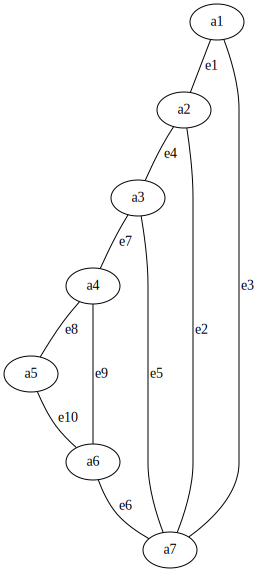
\includegraphics[scale=0.35]{diagrams/Chapter4_Example1.pdf}\\
\end{example*}
Remark: Perfect matching not possible with $\lvert V \rvert$ being odd. 
Maximum cardinality = 3. Empty set is a matching. All subsets of matchings are matchings.
\\
Maximum cardinality:
$\left\{e_{3},e_{1},e_{9}\right\}$
 $\left\{e_{10},e_{5},e_{1}\right\}$\\
Maximal matching:
$\left\{e_{2},e_{9}\right\}$
\begin{lemma}
If $M$ is a matching of maximum cardinality it is a maximal matching.
\end{lemma}
\begin{proof}
Let $M'$ be a matching with $M\subseteq M'$, assume $M \subset M'$ then $\lvert
M' \rvert > \lvert M \rvert \Lightning \:$(as $M$ has maximum cardinality).
\end{proof}
Remark: There are maximum matchings without maximum cardinality.
\begin{lemma}
If $M$ is perfect then $2 \lvert M \rvert = \lvert V \rvert$.
\end{lemma}
\begin{proof}
Obvious.
\end{proof}
\begin{lemma}
If a graph has a perfect matching $M$ then every matching of maximum cardinality is perfect. Clearly, $M$ is
of maximum cardinality.
\end{lemma}
\begin{proof}
Obvious.
\end{proof}
\section{Matching in bipartite graphs}\index{Matching in bipartite graphs}
Problem: Find a matching of maximum cardinality in a bipartite graph.\\
Solution: Construct an associated network as follows:\\
Let $G=(V,E)$ in a bipartite graph.\\ $V = X \cup Y$\\$\overline{V}=V \cup \left\{s,t\right\}$\\
$X\cap Y=\emptyset$\\$\overline{E}=\left\{s \rightarrow x: x \in X \right\}\cup \left\{ y \rightarrow t: y \in Y \right\}$\\
$\overline{c}(\overline{e})=1, \forall \overline{e} \in \overline{E}$
\begin{example*}
\includegraphics[scale=0.7]{diagrams/Chapter4_Example2.pdf}\\
One solution:\\
\includegraphics[scale=0.7]{diagrams/Chapter4_Example3.pdf}\\
\begin{enumerate}
  \item $s$ marked
  \item $x_{1}: \overrightarrow{(s, x_{1})}$
  \item $x_{2}: \overrightarrow{(s, x_{2})}$
  \item $x_{3}: \overrightarrow{(s, x_{3})}$
  \item $x_{4}: \overrightarrow{(s, x_{4})}$
  \item $x_{5}: \overrightarrow{(s, x_{5})}$
\end{enumerate}
Solution:\\
\includegraphics[scale=0.7]{diagrams/Chapter4_Example12.pdf}\\
\end{example*}
\begin{theorem}
The number of edges in a matching $M$ of maximum cardinality coincides with $F_{max}$, i.e. the
 maximum total flow in the associated network.
\end{theorem}
\begin{proof}
Let $M$ be a matching of maximum cardinality. For every edge $x-y$ in $M$ we transport one unit along
the path $s-x-y-t$. We can do that as the edges in $M$ are node disjoint, i.e. they do not share nodes.
This defines a flow function $f'$ with $F'=\lvert M \rvert$ and hence $F_{max}\ge F' = \lvert M \rvert$. 
Now let $f$ be an arbitrary flow function for the associated network, without loss of generality we may choose
$f$ such that $f(e)\in \mathbb{N} \: \forall e$. All paths that connect $s$ with $t$ have the form 
$s \rightarrow x \rightarrow y \rightarrow t$. If such a path is used to transport a unit value then it is clear that
no flow can happen along edges of the form $x \rightarrow y'$ or $x' \rightarrow y$.
\includegraphics[scale=0.7]{diagrams/Chapter4_Example4.pdf}\\
Let $N=\left\{x-y:f(x \rightarrow y)=1\right\}$. $N$ is a matching and the total flow of $f$, i.e. $F$, satisfies
$F=\lvert N \rvert \le \lvert M \rvert$, hence also $F_{max}$, because $M$ was assumed to be of maximum cardinality.
Hence $\lvert M \rvert=F_{max}$ because we chose $f$ arbitrarily. 
\end{proof}
This theorem yields an algorithm to determine
a matching of maximum cardinality. Given a bipartite graph $G=(V,E)$ with $V = X
\cup Y$ and $X \cap Y = \emptyset$:
\begin{enumerate}
  \item Construct the associated network.
  \item On this network, calculate a flow function with maximum total flow.
  \item The matching of maximum cardinality is obtained by $N=\left\{x - y: f(x \rightarrow y) = 1\right\}$.
\end{enumerate}
\begin{definition}
Let $G$ be a bipartite graph, $V = X \cup Y; \: X \cap Y = \emptyset$. Let $A
\subseteq X$. Let $\Gamma(A)= \left\{y \in Y: \exists x \in A: x - y \in E\right\}$. ($\Gamma(A)$: potential partners for the elements in A).
A matching $M$ is called \emph{complete} if $\lvert M \rvert = \lvert X \rvert$, i.e. every $x \in X$ gets a partner.
\end{definition}
\begin{theorem}
Wedding or marriage theorem: A bipartite graph has a complete matching if and only if for every $A \subseteq X$
$\lvert \Gamma(A) \rvert \ge \lvert A \rvert$.
\end{theorem}
\begin{proof}
``>'' Let G have a complete matching $M$, let $A \subseteq X$. Then every $x \in X$ has a partner for itself in $M$,
hence for every $A \subseteq X \lvert \: \Gamma(A) \rvert\ge \lvert A \rvert$. \\
``<'' Let $\lvert \Gamma (A) \rvert \ge \lvert A \rvert$ for every $A \subseteq X$. Assume there is no complete
matching. Let $S$ be the set of nodes that were marked in the last step of Ford-Fulkerson in the associated 
network. The calculated flow function determines a matching $M$ with i) $F=\lvert M \rvert$. As we assumed that there
is no complete matching we get ii) $\lvert M \rvert < \lvert X \rvert$.\\
\includegraphics[scale=0.45]{diagrams/Chapter4_Example5.pdf}\\
Marking in the last round of Ford-Fulkerson. $S=$ the marked nodes.\\
$A:=X \cap S$\\
Let $y \in \Gamma (A)$ then there is an $x \in A = \: X \cap S \: x$ marked and $x-y$ is an edge in $E$.\\
In the last successful construction of an augmenting path there was no flow determined along the edge $s \rightarrow x$,
otherwise we could not mark $x$ now. Hence the flow along the edge $x \rightarrow y$ must have been $0$ before 
as well. Hence the remaining capacity $x \rightarrow y \: = 1$.
\section{Stable matching (marriage)}\index{Stable matching (marriage)}
Given:\\ 
1. n men $b_{1} \dots b_{n}$, n women $a_{1} \dots a_{n}$\\
2. each person has a preference list of the other sex: \\
$a_{1}: b_{2}, b_{3}, b_{1} \dots$, where $a_{1}$ likes $b_{2}$ best.
\end{proof}
Task: Form couples respecting the preferences.\\
A matching or coupling associates with each man exactly one woman. A matching is called \emph{unstable} if there is a man $a$ and a woman $A$ such that:
$a$ prefers $A$ to the woman $B$ he is matched with and $b$ prefers $B$ to the woman $A$ he is matched with.
A matching is called \emph{stable} if it is not unstable.\\
Given n men, n women. Here are two approaches:\\\\
\underline{1. Attempt: Try all possible matchings}\\
%[INSERT MISSING ILLUSTRATION!]
There are $n!$ possible matchings. There are therefore ${n \choose k} =
O(n^2)$ checks to find out if one given matching is stable altogether $O(n! * n^2)$.
For n=10 this equals 300,000,000 checks.\\\\
\underline{2. Gale-Shapley Algorithm}
\begin{enumerate}
\item{Mark every person as ``free''.}
\item{As long as there is a free man m do: Let F be the first woman to which m has not yet made an offer. If F is 
free then match m with F ((F,m)) and mark both as ``bound''. If F is bound to m' then check if F prefers
m to m'. If this is so, substitute the pair (F, m') by (F.m). Mark m' as free and m as ``bound''.\\If F does not
prefer m to m' then nothing is changed.}
\item{Output all pairs.}
\end{enumerate}
\underline{Statement:} For any input the algorithm terminates and yields a
stable matching.\\
\emph{1. Observation:} It cannot happen that a man is rejected by all
women.
This is because if a woman rejects or leaves a man she is bound.
When the man reaches the end of his list then all women would be bound.
\Lightning because there are $n$ women and $n-1$ other men. \\
\emph{2. Observation:} The algorithm consists of offers made by men. Each
man makes at most n offers $\implies O(n^2)$ offers in the worst case. \\
\emph{3. Observation:} The result is a matching because the algorithm
terminates when all men are bound and every man is bound to exactly one woman. \\
\emph{4. Oberservation:} The resulting matching is stable. Assume this is
not the case.\\
$m$: $F' \dots F$ \\
$F'$: m \dots m' \\
$F$ matched with $m$. \\
$F'$ matched with $m'$. \\
m makes offers according to his list. So he made an offer to F' before he
reached F.\\
\emph{Case 1}: $F'$ was free. So she accepted his offer, but later
left him.
This can only happen because of men she likes better than $m$, but $m'$ could not break
into such a marriage. \\
\emph{Case 2}: $F'$ was bound. \\
\emph{Case 2.1}: $F'$ was bound to a partner she prefers to $m$,
then she does not leave this partner because of $m$ and def. not because of $m'$.\\
\emph{Case 2.2}: $F'$ leaves her partner because of $m$, but $m'$
cannot break into this marriage. \\
Hence the matching is stable. The cost of the algorithm is $O(n^2)$. \\
$n=10$: algorithm takes 100 Steps; trying all takes 300,000,000 steps. \\
$n=1009$: algorithm takes $10^6$ steps;  trying all takes $500^500$ steps. Age
of planet earth: $4*10^9$ years.\\
A man and a woman $F$ are called \emph{stable partners} if there is a stable
matching in which they are bound to each other. \\
\emph{Statement:} All executions of the algorithm yield the same result. In this
matching each man gets the best partner he can get in any stable matching. Let E
be an arbitrary execution of the algorithm, let the result be the matching
$M_{E}$. Assume there is another matching $M$.\\
$M_{E}$: $m - F$ \\
$M$: $m - F'$ \\
$m$: $\dots F' \dots F \dots$ \\
Then deriving $E$, $F'$ must have rejected / left $m$. Without loss of
generality, let this be the first time that a woman rejected / left a stable
partner. Let $m'$ be the reason for this.\\
$F'$: $\dots m' \dots m \dots$ \\
Then $m'$ cannot have a stable partner he prefers to $F'$, hence $m'$ prefers
$F'$ to his partner in $M$.\\
$M$: $m - F'$; $m' - F''$\\
So $M$ is not stable.

\section{Maching in general graphs}
\label{sec:Matching in general graphs}
 \begin{example*}
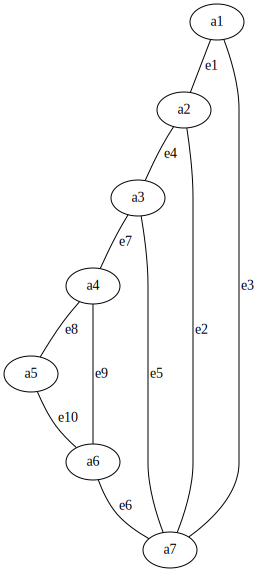
\includegraphics[scale=0.35]{diagrams/Chapter4_Example1.pdf}\\
\end{example*}
$\{e_{1}, e_{5}, e_{9}\}, \: \{ e_{1}, e_{5}, e_{10}\}$ are both matchings of
maximal cardinality because $|V|=7$.\\
Every subset of a matching is a matching.
\begin{example*}
\includegraphics[scale=0.35]{diagrams/Chapter4_Example6.pdf}\\
\end{example*}
$M_0=\{\{V_{2}, V_{3}\}, \{V_{4}, V_{5}\}, \{V_{7}, V_{10}\}\}$
\begin{definition}
	Let $G=(V,E)$ be a graph and $M$ a matching for $G$. The edges in $M$ are
	called ``matched'', the others are called ``free''. If $\{u,v\} \in M$ then
	$u,\:v$ are called partners and ``matched''. If $v \in V$ lies on no edge of
	$M$ then $v$ is called ``free''. A simple path $e_{1}, e_{2}, \dots, e_{k}$ is
	called $M$-alternating if $e_{1}, e_{3}, e_{5} \dots$ are free eges and
	$e_{2}, e_{4}, \ldots$ are matched.\\
		\includegraphics[scale=0.5]{diagrams/Chapter4_Example7.pdf}\\
		\\
	An $M$-alternating path is called $M$-augmenting if the start and end points of
	the path are free.
\end{definition}
\begin{lemma}
	If p is an $M$-augmenting path, $p=e_{1}, \dots, e_{l}$, then $l$ is odd and
	the number of nodes in the path is even.
\end{lemma}
\begin{proof}
	As the first and last node on an $M$-augmenting path must be free, the first
	and last edge must be free edges.\\
	$\frac{e_{1}}{free} \: \frac{e_{2}}{free} \: (e_{1} \: e_{2})(e_{3} \: e_{4})
	\dots$ \\
	Assume $l$ is even, then we can group the edges into pairs $ (e_{1} \:
	e_{2})(e_{3} \: e_{4}) \dots$ and so on and the last edge would then be
	matched.\\ \emph{Contradiction:} In a simple path of odd length the number of
	nodes is even.\\
\end{proof}
\begin{lemma}
	Let $G=(V,E)$ be a graph, $M$ a matching and $p$ an $M$-augmenting path. Then
	$M'=M \smallsetminus p \cup p \smallsetminus m$ is a matching and $|M'| =
	|M|+1$.
	(See ex. $E$ and $M_{0}$). \\
\end{lemma}
\begin{itemize}
	\item{$p=v_{6} - v_{8}$\\$M_{0}$-alternating? Yes \\$M_{0}$-alternating? Yes}
	\item{$p'=v_{1} - v_{2}$\\$M_{0}$-alternating? Yes \\$M_{0}$-alternating? No}
	\item{$M_{1} = M_{0} \smallsetminus p \cup p \smallsetminus M_{0} = \{\{v_{2}, v_{3}\},
	\{v_{4}, v_{5}\}, \{v_{7}, v_{10}\}, \{v_{6}, v_{8}\}\}$}
	\item{$p_{1}: v_{1} - v_{2} - v_{3} - v_{5} - v_{4} -
	v_{8}$\\$M_{1}$-alternating? Yes \\ $M_{1}$-alternating? No}
	\item{$p_{2}: v_{1} - v_{4} - v_{5} - v_{6} - v_{8} -
	v_{7} - v_{10} - v_{9}$\\$M_{1}$-alternating? Yes \\ $M_{1}$-alternating? Yes}
	\item{$M_{1} = M_{1} \smallsetminus p_{2} \cup p_{2} \smallsetminus M_{1} = \{\{v_{2},
	v_{3}\}, \{v_{1}, v_{4}\}, \{v_{5}, v_{6}\}, \{v_{8}, v_{7}\}, v_{10},
	v_{9}\}\}$}\\ $|M_{2}| = 5$ is of maximum cardinality as there are 10 nodes.
\end{itemize}
\begin{proof}
Let $p$ be an $M$-augmenting path. \\$p$: $v_{1} - v_{2} - v_{3} \dots -
v_{2k}$\\
Show 1. $M'$ is a matching $(M' = M \smallsetminus p \cup p \smallsetminus M)$, i.e. no two
edges share a node. Assume there are two edges in $M'$ that share a node, $e$
and $e'$. There are 3 cases to consider:\\
i) $e, e' \in M \smallsetminus p$ \\
ii) $e, e' \in p \ M$  \\
iii) $e \in M \smallsetminus p, e' \in p \smallsetminus m$ \\
\emph{Case i)} $e, e'$ share a node and are in $M \smallsetminus p$, in particular $e,
e' \in M \: \lightning $ \\
\emph{Case ii)} $e, e' \in p \smallsetminus M$, in particular $e, e' \in p$ and not in
$M$. But on $p$ only edges share a node if one is in $M$ and the other isn't. \\
\emph{Case iii)} Let $e \in M \smallsetminus p, \: e' \in p \smallsetminus M$,
i.e. $e'$ is free. 
\begin{example*}
		\includegraphics[scale=0.65]{diagrams/Chapter4_Example8.pdf}\\
\end{example*}
Without loss of generality, assume that $v_{2j}$ also lies on $e$. \\
$e''$ is in $M$, hence $e, e'' \in M$ and share a node. $\lightning$. (If
$v_{2j}$ is the last node, use $v_{2j-1}$ for a similar argument.) \\
Show 2. $|M'| = |M| + 1$ \\
$p$: $v_{1} - v_{2} \dots v_{2k-1} - v_{2k}$, where $\{v_{1}, v_{2}\}$ and
$\{v_{2k-1}, v_{2k}\}$ are not in $M$. \\
$p$ contains $2k-1$ edges and $k-1$ belong to $M$ and $k$ do not belong to $M$.\\
$e_{1}, e_{3}, \dots, e_{2k-1}$ \\
$|(M \smallsetminus p) \cup (p \smallsetminus m)| = |M \smallsetminus p| + |p \smallsetminus M|\\ =
|M| - (k-1) + k \\ = |M| + 1$\\
\end{proof}
\begin{lemma}
	$G=(V,E)$ graph, $M$ matching, $u\in V$ free. Let us assume that there is no
	$M$-augmenting path starting in u. Let $p$ be an $M$-augmenting path with end
	points $v, w$. Then there will be no $(M \smallsetminus p \cup p \smallsetminus
	)$-augmenting path starting from $u$.
\end{lemma}
\begin{lemma}
A matching $M$ is of max. cardinality if and only if there is no $M$-augmenting
path.
\end{lemma}

\begin{proof}
``>'' Let $M$ be of max. cardinality. Assume there is an augmenting path, then
construct $M'=M \smallsetminus p \cup p $ and $|M'| > |M| \lightning$. \\
``<'' Let there be no $M$-augmenting path. Assume that there is a matching $M'$
with $|M'| > |M|$. Consider the edges in $M \smallsetminus M' \cup M' \smallsetminus M$.
$G' = (V, (M \smallsetminus M') \cup (M' \smallsetminus M))$. In this graph every node has 
degree 2 or less. If $v$ has degree 2, then one edge belongs to $M$, the other
to $M'$. Two connected components of $G'$ are either paths or circles. \\
		\includegraphics[scale=0.5]{diagrams/Chapter4_Example9.pdf}
\\or\\
		\includegraphics[scale=0.5]{diagrams/Chapter4_Example10.pdf}\\
where the number of edges in the circle belonging to $M$ equals the number of
edges
belonging to $M'$. As $|M'| > |M|$ and the circle cannot contribute to this
fact, we conclude that there must be a path with more edges in $M'$ than in $M$.
This path must look like this:
\includegraphics[scale=0.5]{diagrams/Chapter4_Example11.pdf}\\
$\lightning$
\end{proof}
Here is an idea for an algorithm which finds a matching of maximal cardinality:
\begin{enumerate}
  \item {Start with an initial matching, e.g. consisting of one edge}
  \item {Find an M-augmenting path. Put $M = M \smallsetminus p \cup p \smallsetminus
  M$. Go to 2. If there is no M-augmenting path, stop; the current matching is
  of maximal cardinality.}
\end{enumerate}

\chapter{Networks with costs, respectively upper/lower bounds}

\section{Networks with costs}\index{Networks with costs}

Get rid of parallel and antiparallel edges, cost: $E \rightarrow \mathbb{R}$ 

\begin{example}
\underline{case a)}\\

\begin{figure}[h]
\includegraphics[scale=0.45]{diagrams/graph5_1}
\caption{With antiparallel edges}
\label{G1}
\end{figure}

\begin{figure}[h]
\includegraphics[scale=0.45]{diagrams/graph5_2}
\caption{With antiparallel edges}
\label{G2}
\end{figure}

\ref{G1} is transformed to \ref{G2}
\\
$c(e{_1})$ as before $c$.\\
$cost(e{_21}) = cost(e{_2})$\\
$cost(e{_22}) = 0$\\
$cost(e{_21}) = cost(e{_22}) = cost(e{_2})$\\

\underline{case b)}\\

\begin{figure}[h]
\includegraphics[scale=0.45]{diagrams/graph5_1}
\caption{With antiparallel edges}
\label{fig:G3}
\end{figure}

\begin{figure}[h]
\includegraphics[scale=0.45]{diagrams/graph5_3}
\caption{After transformation - without antiparallel edges}
\label{fig:G4}
\end{figure}

\ref{fig:G3} is transformed to \ref{fig:G4}\\
\end{example}

From now on we consider only networks without parallel/antiparallel edges.

\begin{definition}
Let $G=(V,E)$ with $s, t \in V, c: E \rightarrow \mathbb{R^+}$ be a network. Let cost: $E \rightarrow \mathbb{R}$ be a function that associates ``cost'' to every edge.
Let f be a flow function for this network. \\

$cost(f) = \sum\limits_{e \in E} f(e) * cost(e)$\\

\end{definition}


\textbf{Task:}\\
Given:
\begin{enumerate}
  \item a network $G=(V,E), s, t \in V, c, cost$
  \item $w \in \mathbb{R^+}$
\end{enumerate}
Find a flow function f with total flow $F=w$ and minimal costs.


\begin{definition}
$G=(V,E), s, t \in V, c, cost, f flowfunction$\\
The graph $G{_f}=(V,E{_f})$ with $\tilde{c}$, $\tilde{costs}$.\\
Let $e=(u,v) \in E$
\begin{enumerate}
  \item If $f(e) < c(e)$ then $e{_1}=(u,v) \in E{_f}$\\
  $\tilde{c}(e{_1}) = c(e) - f(e) > 0 $\\
  $\tilde{cost}(e{_1}) =  cost(e)$\\
  \item If 0 < $f(e)$ then $e{_2}=(v,u) \in E{_f}$\\
   $\tilde{c}(e{_2}) = f(e)$\\
   $\tilde{cost}(e{_2}) =  - cost(e)$\\
\end{enumerate}
\end{definition}

\textbf{Observation:}\\
\begin{enumerate}[label=\alph*]
  \item 
  If $e \in E$ is an edge with $0 < f(e) < c(e)$\\
\begin{figure}[h]
\includegraphics[scale=0.45]{diagrams/graph5_4}
\caption{$G=(V,E)$}
\label{fig:G5}
\end{figure}  
\begin{figure}[h]
\includegraphics[scale=0.45]{diagrams/graph5_1}
\caption{$G{_f}$}
\label{fig:G6}
\end{figure}    

\item 
If $e \in E$ is an edge with $0 < f(e) = c(e)$ - as shown in \ref{fig:G7}.
\begin{figure}[h]
\includegraphics[scale=0.45]{diagrams/graph5_5}
\caption{$G{_f}$}
\label{fig:G7}
\end{figure}

\item
If $e \in E$ is an edge with $0 = f(e) < c(e)$ - as shown in \ref{fig:G8}.
\begin{figure}[h]
\includegraphics[scale=0.45]{diagrams/graph5_6}
\caption{$G{_f}$}
\label{fig:G8}
\end{figure}

\item 
If $e \in E$ is an edge with $0 = f(0) = c(0)$ - as shown in \ref{fig:G9}.
\begin{figure}[h]
\includegraphics[scale=0.45]{diagrams/graph5_7}
\caption{$G{_f}$}
\label{fig:G9}
\end{figure}
\end{enumerate}

\begin{definition}
Let p be a directed cycle in $G{_f}$.
$cost (p) := \sum\limits_{e \in P} cost(e)$
\end{definition}

\begin{example}

\begin{figure}[h]
\includegraphics[scale=0.45]{diagrams/graph5_8}
\caption{$G$}
\label{fig:G10}
\end{figure}

\begin{figure}[h]
\includegraphics[scale=0.45]{diagrams/graph5_9}
\caption{$G{_f}$}
\label{fig:G11}
\end{figure}

directed cycles of negative costs:
$t - h - b - d - t \rightarrow -1$\\
$s - c - g - h- b - a - s \rightarrow -5$\\
\end{example}


\textbf{Theorem 5.1}\\
Let a network with cost function be given and a flow function f with total flow $F=w$. $f$ has least costs among all flow functions with total flow $w$ if and only if $G{_f}$ does not have any directed cycles of negative cost.

\begin{proof}
``$\implies$'' Let f be a cost minimal flow function with total flow $F=w$. Assume that $G{_f}$ contains a directed cycle of negative costs. Adapting the flow values along this cycle in the original network we can reduce the cost while maintaining the total flow.
\end{proof}

\begin{example}

\begin{figure}[h]
\includegraphics[scale=0.5]{diagrams/graph5_10}
\caption{$G{_f}$}
\label{fig:G12}
\end{figure}

\begin{figure}[h]
\includegraphics[scale=0.5]{diagrams/graph5_11}
\caption{$G{_f}$}
\label{fig:G13}
\end{figure}


For edges that correspond to forward edges (of type $e{_1}$) we may raise the flow value.
For edges that correspond to backward edges (of type $e{_1}$) we may reduce the flow.

\end{example}
\chapter{NP-Completeness}

\begin{descr}
  Definition and analyisis of different complexity classes
\end{descr}

\section{Motivation/Examples}
\begin{tabular}{p{5cm}|p{5cm}}
  Solvable in Polinomial Time & NP complete \\
  \hline
  \deftxt{Euler Path} "a path with all edges" & \deftxt{Hamiltonian Path} "node ocurs exactly once" \\
   Shortest path from X to Y $\Rightarrow$ \deftxt{Dijkstra's}algorithm & longest simple Path between X and Y \\
  \hline
  2-CNF (conjuntive normal form) e.g. $(x_{1} \lor \lnot x_{2}) \land (\lnot x_{1} \lor x_{3})$ Can we find an assignment, that the formula becomes true in poly. time? & 3-CNF \\
  \hline
  Two processor scheduling & 3 or more processor schedulung $\Rightarrow$ NP-complete or unknown \\
  \hline
  Football game until 1955 loss 0 points, draw 1 point, win 3 points. The season has already started, is my team still able to win the championchip? & loss 0 points, draw 1 point, win 3 points \\
\end{tabular}

\section{Introduction}
\begin{definition}
  P is the class of problems that can be solved in polinomial time.\\

  NP is the class of porblems, where given a solution one may check in polinomial time, that it is indeed one.
\end{definition}

\begin{example}
Example:
\begin{enumerate}
  \item Given a connected undirected-finite graph. Is there a circle such taht every node appears exatly once on the circle.
        Given such a circle $< v_{1},...v_{n}>$ it can easily checked that it has the property. $\Rightarrow$ Hamiltonian Cycle $\in$ 
        NP.
  \item 3-CNF; given values for the variables, we can check that the formula becomes true, with this values in polynomial time.
\end{enumerate}

\textbf{Clarity:} $P \subseteq NP$ open problem; $P = NP ??$

Overview: \\
\includegraphics[scale=0.3]{diagrams/comp_classes}
\end{example}

\section{Problem Types/Issues}

\begin{tabular}{p{5cm}|p{5cm}}
  \textbf{Decision Problems} & \textbf{Optimization Problems} \\
  \hline
  Yes or no answer, is there a path from X to Y? & Find the shortest path from X to Y?
\end{tabular}

\begin{definition}
  Complexity Theory deals with \deftxt{decision problems}. Optimization problems are tried to transform into decision problems.
\end{definition}

\begin{example}
  Choose an integer k, treat the decision problem: "Is there a path from X to Y no longer than k?"
\end{example}  

To show that an optimization problem is hard to solve it is sufficient to consider the related decision problem. If the latter is hard to solve, so is the first. \\

\textbf{Reductions} \\
Reductions are used to show that problem are hard to solve. A reduction reduces a decision problem to another one.\\
$A \Rightarrow B$ (reduction)

Properties of the reduction should be: "it can be done in polynomial time". \\
If $A$ and $B$ the transformation of $A B$ is an instance of $B$ then $A$ should have the answer yes if and only if $\beta$ has the answer yes.\\
Call this a \deftxt{polynomial reduction}.\\
If $A \rightarrow B$ and $B$ can be solved in poly. time, then instances of $A$ can be solved in poly. time. \\
If $A \rightarrow B$ and $A$ is hard to solve, then we may conclude that  $B$ is hard to solve. \\


\chapter{Approximation Algorithms}
An algorithm for an optimization problem that yields a ``nearly''
optimal solution is called an approximation algorithm.
$0<C_{n}*$ cost of an optimal solution for an input of size
$n$ (e.g. length of a shortest path). $0<C_{n}$ cost of a solution
produced by an approximation algorithm. If 
$max(\frac{C_{n}}{C_{n}*},\frac{C_{n}*}{C_{n}})=\rho (n)$ then
the algorithm has an approximation ratio of $\rho (n)$.\\
(Remark: $\rho (n) \ge 1$)\\
$\rho (n) = 1$: optimal, $\rho(n) >> 1$: bad approximation\\
Trade-off: Cost of the approximation algorithm vs. quality of approximation.\\
An approximation scheme for an approximation problem is an 
algorithm with 2 inputs: $Problem + \epsilon>0$ such that
the algorithm is a $(1 + \epsilon)$ - approximation algorithm.\\
The approximation scheme is a polynomial time approximation
scheme if for each $\epsilon > 0$ the induced algorithm runs in polynomial time in $n$.
It is fully polynomial if it is polynomial in $n$ and in $1/\epsilon$.
\begin{example}
$O(n^(\frac{2}{3}))$, if $\epsilon' = \frac{3}{4}$ $O(n^(\frac{8}{\epsilon}))$ cost, i.e.
the costs are rising but not by a constant factor.
\end{example}
\begin{example}
$O((1/\epsilon)^2 * n^3)$ fully polynomial. $\epsilon = \frac{\epsilon}{4}
O(16*(\frac{1}{\epsilon}^2 * n^3))$.
\end{example}
\section{Heuristic Approaches}
\emph{Vertex Cover}: Given an undirected graph $G=(V,E)$ without parallel edges and without loops,
we look for a minimal set $V'$ of nodes such that each edge has at least one endpoint in $V'$.
\begin{example*}
\includegraphics[width=\textwidth]{diagrams/Chapter7_Example1.pdf}
\end{example*}
\begin{algorithm}
\begin{algorithmic}[1]
\State $C \gets \emptyset$
\State $E' \gets E$
\While{$E' \neq \emptyset$}
	\State Choose an edge $\{u,v\}$ in $E'$.
	\State $C \gets C \cup \{u,v\}$
	\State Remove all edges from $E'$ with the end point $u$ or $v$.
\EndWhile
\end{algorithmic}
\caption{APPROX-VERTEX-COVER($G=(V,E)$)}
\end{algorithm}

\section{Probabilistic Analysis and randomized algorithms}

\textbf{Assistant search}
\begin{enumerate}
  \item[1] best = 0
  \item[2] for i = 1 .... n do\\
\noindent\hspace*{10mm}	interview candidate i\\
\noindent\hspace*{10mm}	if candidat i is better than best\\
\noindent\hspace*{20mm}		then best:= i\\
\noindent\hspace*{20mm}		employ candidate i (fire previous candidate)\\
\end{enumerate}

\underline{Analysis} of the cost that arise from interviews and hiring.\\
cost of an interview $c{_I}(low)$\\
cost of hiring: $c{_E}(high)$\\
Cost that arise in the worst case $O(n* c{_I} +  m * c{_E}$ ) if m people are hired 
and \\
$O(n * c{_I} +  n *  c{_E} )$ if n people are hired \\
worst case: if candidates show up in the order: worst first, \ldots best last

\textbf{Indicator Variable}
Let S be a set and $A \subseteq S$ and execute the indicator variable.\\

$ X(s)=\left\{\begin{array}{cl} 1, if s\in A \\ 0, else \end{array}\right .$

$E[x{_1}] = \sum\limits_{x} x Pr(X{_A}=x) = Pr(A)$

\textbf{Example}
Throw a coin n times.
$ X(s)=\left\{\begin{array}{cl} 1, \mbox{ if in the i-th throwing head is shown} \\ 0, \mbox{  otherwise } \end{array}\right .$

$S = {(a{_1},\ldots,a{_n}) : a{_i} \in {H,N}}$,
Let X be the random variable that describes how often ``H'' appears when you throw n-times.

$X:\{H,N\}^n \rightarrow \mathbb{N}$
$X=\sum x{_i}$

The expected number of ``H''\\

$E[X] = E[\sum x{_i}] = \sum\limits_{i=1}^n E[x{_i}] = \sum\limits_{i=1}^n \frac{1}{2} = \frac{n}{2}$

\textbf{Example Hiring:}\\

$ X{_i} = \left\{\begin{array}{cl} 1, \mbox{ if the candidate is hired} \\ 0, \mbox{  else } \end{array}\right .$

$X= \sum\limits_{i=1}^n x{_i}$ describs how many candidates are hired\\

$E[X] =  E[\sum\limits_{i=1}^n x{_i}] = \sum\limits_{i=1}^n E[x{_i}]$\\

$E[X{_i}] = $ Probability that the i-th candidate is hired.


Candidate i is hired if this person is better than the first i-1 candidates. If the order in which people are chosen is random, each of the first i candidates is the best with same probability.
So $E[x{_i}] =\frac{1}{i}$\\
$E[X] =  \sum\limits_{i=1}^n \frac{1}{i} = \ln n + O(1)$ 


\begin{lemma}
If the order in which the candidates appear is random then the average cost of finding a suitable employee is
$ O( c_E *  \ln n + C_I * n)$
\end{lemma}

\textbf{Question:}
How can we know that the order is random ?\\

\subsection{Randomized Algorithms}
In order to guarantee randomness of the input, we randomize it. 

\begin{example}{Hiring}
Given the list of the n candidates, use random numbers to select a candidate for an interview.
$RANDOM(a,b)$ produces an integer z with  $a \leq z \leq b$ where all numbers in this interval are equally probable. 
$RANDOM(0,1)$ produces 0 or 1 with equal probability $\frac{1}{2}$
$RANDOM(3,7)$ produces 4 with probability $\frac{1}{5}$ \\
\end{example}
  
\textbf{Randomized-Assistant Search}
\begin{enumerate}[label={\arabic*.}]
 \item Permute the list of candidates using a  random number generator
 \item best = 0
 \item ... as before
\end{enumerate}

\begin{lemma}
The expected cost for hiring using the randomized assistant search algorithm is \\
$O( c_E * \ln n + C_I * n)$
\end{lemma}
How to randomize an in input of n elements [A[1...n]]? \\
PERMUTE-BY-SORTING(A) \\
1.	n = length(A) \\
2.	for i = 1...n do \\
3.	P[i] = RANDOM [1, $n^3$] (something arbitrary bigger than n) \\
4.	Sort the array A using P as sort keys \\
5.	return A \\
\newline
RANDOMIZE-IN-PLACE(A) \\
1.	n = length(A) \\
2.	for i= 1...n do \\
3.	  swap A[i] $\Leftrightarrow$  A[RANDOM(i,n)] \\
>>>>>>> 537543df52b95855cfa2f207fc7482bd87d8b8b6




\appendix
\chapter*{ Appendix 4: Application of general matching}

\section{Two processor scheduling}\index{Two processor scheduling}

Given:\\
\begin{enumerate}
  \item Two identical agents/processors
  \item Collection of n jobs or taskstogether with a directed acyclic graph with n nodes which correspond to the jobs, that describe the preceedence among the jobs.
\end{enumerate}


\begin{example}
2 Graphics missing

\end{example}

How can the jobs be scheduled on the two processors such that the jobs are completed as quickly as possible?

\textbf{Solution}:\\
using matching!\\
\underline{But:}\\
for three processors the problem is NP-Complete.\\

To solve the two processors problem we proceed as follows. We construct a graph $G*$ thathas the same nodes as $G$ and there is an edge {x,y} in $G*$ if and only if there is no path from x to y in $G$ and no path from y to x in $G$.

\underline{1. Observation:}\\
if we have a schedule we can obtain a matching. If the schedule is optimal the matching is of maximal cardinality.

\underline{2. Interessting:}\\
We can use matching of maximal cardinality to produce a schedule that is optimal.\\

Let S be a set of nodes with indegree 0. Let $M*$ be a matching of max. cardinality for $G*$. Apply the following rules repeatly:\\
\begin{enumerate}
  \item If there is an unmatched node in S then schedule it. Remove it from G.
  \item If there is a pair of jobs in S that are unmatched in $M*$then we schedule this pair in the output and delete the two nodes (corresponding to the jobs) in G.
\end{enumerate}

If neither rule 1 nor rule 2 applies and there are still jobs left to be scheduled then we know that S contains only nodes thatare matched
and for every node in S its partner ($M*$) is not in S.\\

$J{_1} \in S$ ------$M*$------
$J'{_1} \notin S$\\

$J{_2} \in S$ ------$M*$------
$J'{_2} \notin S$\\

Observation:\\
$\not\exists$ path $J_{1}$ to $J_{2}$ 





% ================================

\ifthenelse{\equal{\useThumbs}{1}}
	{\ihead[]{}}{}
\ifthenelse{\equal{\useIndex}{1}}{
\clearpage
\renewcommand{\indexname}{Index}
\printindex}{}
\end{document}